\section{Автономный генератор}

Для того, чтобы привести систему
\begin{equation}
    \begin{cases}
        \dot{x} = Ax \\ 
        g(t) = Cx
    \end{cases}
    \label{eq:system3}
\end{equation}
к желаемому виду $\cos(4t) + e^{-8t}\cos(5t)$
Представим $g(t)$ в виде:
\begin{equation}
    g(t) = \frac{1}{2}e^{4it} + \frac{1}{2}e^{-4it} + \frac{1}{2}e^{-8 + 5it} + \frac{1}{2}e^{-8 - 5it}
\end{equation}
Можно заметить 4 комплексные моды. Отсюда легко понять корни характеристического уравнения:
\begin{equation}
    \begin{cases}
        \lambda_{1, 2} = \pm4i \\ 
        \lambda_{3, 4} = -8 \pm 5i \\ 
    \end{cases}
\end{equation}
Собственные числа матрицы $A$ явлюятся корнями характеристического уравнения. Таким образом, матрица $A$ будет иметь вид:
\begin{equation}
    A = \begin{bmatrix}
        0 & 4 & 0 & 0 \\
        -4 & 0 & 0 & 0 \\
        0 & 0 & -8 & 5 \\
        0 & 0 & -5 & -8
    \end{bmatrix}
\end{equation}
Решив первое дифференциальное уравнение из системы \ref{eq:system3} получим:
\begin{equation}
    x(t) = e^{At} x(0)
\end{equation}
Найдем матрицу $e^{At}$:
\begin{equation}
    e^{At} =  \begin{bmatrix}
        \cos\left(4t\right) & \sin\left(4t\right) & 0 & 0 \\
        -\sin\left(4t\right) & \cos\left(4t\right) & 0 & 0 \\
        0 & 0 & e^{-8t}\cos\left(5t\right) & e^{-8t}\sin\left(5t\right) \\
        0 & 0 & -e^{-8t}\sin\left(5t\right) & e^{-8t}\cos\left(5t\right)
    \end{bmatrix}
\end{equation}
В соответствии со вторым уравнением из системы \ref{eq:system3} выход $g(t)$ будет равен:
\begin{equation}
    g(t) = C e^{At} x(0)
\end{equation}
\begin{equation}
    g(t) = \begin{bmatrix}
        c_1 & c_2 & c_3 & c_4
    \end{bmatrix} \times
    \begin{bmatrix}
        \cos\left(4t\right) & \sin\left(4t\right) & 0 & 0 \\
        -\sin\left(4t\right) & \cos\left(4t\right) & 0 & 0 \\
        0 & 0 & e^{-8t}\cos\left(5t\right) & e^{-8t}\sin\left(5t\right) \\
        0 & 0 & -e^{-8t}\sin\left(5t\right) & e^{-8t}\cos\left(5t\right)
    \end{bmatrix} \times
    \begin{bmatrix}
        x_1(0) \\
        x_2(0) \\
        x_3(0) \\
        x_4(0)
    \end{bmatrix}
\end{equation}
\begin{equation}
    g(t) = \begin{bmatrix}
        c_1 \cos\left(4t\right) - c_2 \sin\left(4t\right) \\
        c_1 \sin\left(4t\right) + c_2 \cos\left(4t\right) \\
        c_3 e^{-8t}\cos\left(5t\right) - c_4 e^{-8t}\sin\left(5t\right) \\
        c_3 e^{-8t}\sin\left(5t\right) + c_4 e^{-8t}\cos\left(5t\right)
    \end{bmatrix}^{T} \times
    \begin{bmatrix}
        x_1(0) \\
        x_2(0) \\
        x_3(0) \\
        x_4(0)
    \end{bmatrix}
\end{equation}
Для того, чтобы $g(t)$ принял вид $\cos(4t) + e^{-8t}\cos(5t)$, необходимо решить систему 
\begin{equation}
    \begin{cases}
        c_1 x_1(0) + c_2 x_2(0) = 1 \\
        c_3 x_3(0) + c_4 x_4(0) = 1 \\
        c_1 x_2(0) - c_2 x_1(0) = 0 \\
        c_3 x_4(0) - c_4 x_3(0) = 0
    \end{cases}
\end{equation}
Предполагая $c_1=0~,c_2\ne0,c_3=0,c_4\ne0$, получим общее решение: 
\begin{equation}
    x(0) = \begin{cases}
        0 \\
        \frac{1}{c_2} \\
        0 \\
        \frac{1}{c_4}
    \end{cases}
\end{equation}

Примем 
\begin{equation}
    C = \begin{bmatrix}
        0 & 1 & 0 & 1
    \end{bmatrix}
\end{equation}
\begin{equation}
    x(0) = \begin{bmatrix}
        0 \\
        1 \\
        0 \\
        1
    \end{bmatrix}
\end{equation}
Схема автономного генератора представлена на рисунке \ref{fig:autonomous_generator}.
Результат моделирования представлен на рисунке \ref{fig:autonomous_generator_simulation}.

\begin{figure}[ht!]
    \centering
    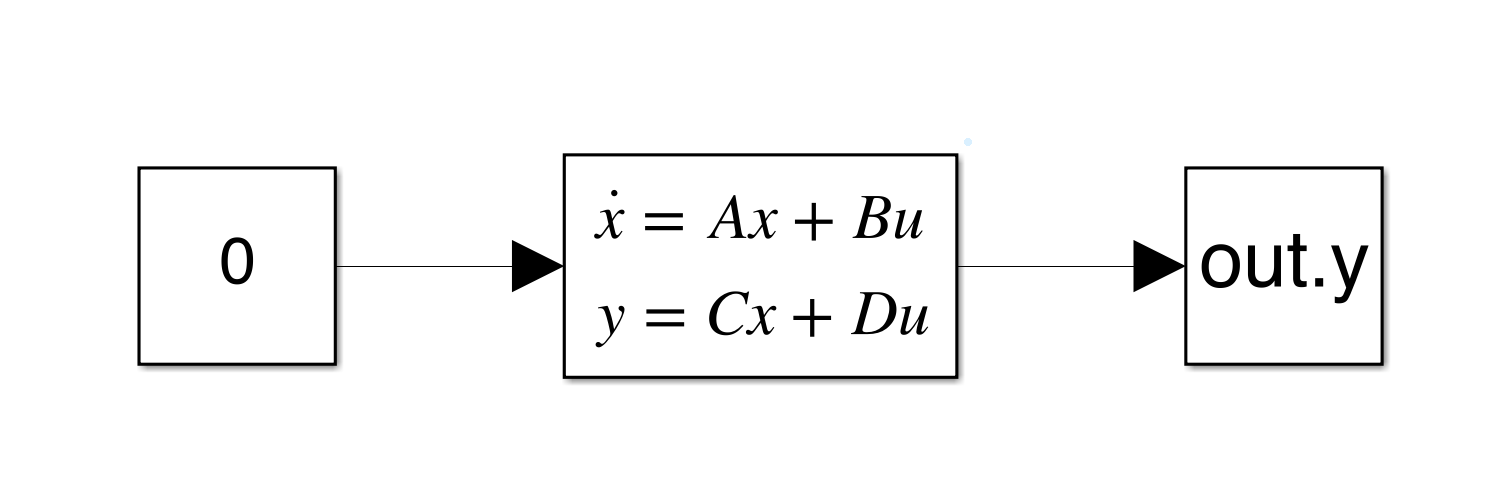
\includegraphics[width=0.8\textwidth]{media/scheme3.png}
    \caption{Схема автономного генератора}
    \label{fig:autonomous_generator}
\end{figure}

\begin{figure}[ht!]
    \centering
    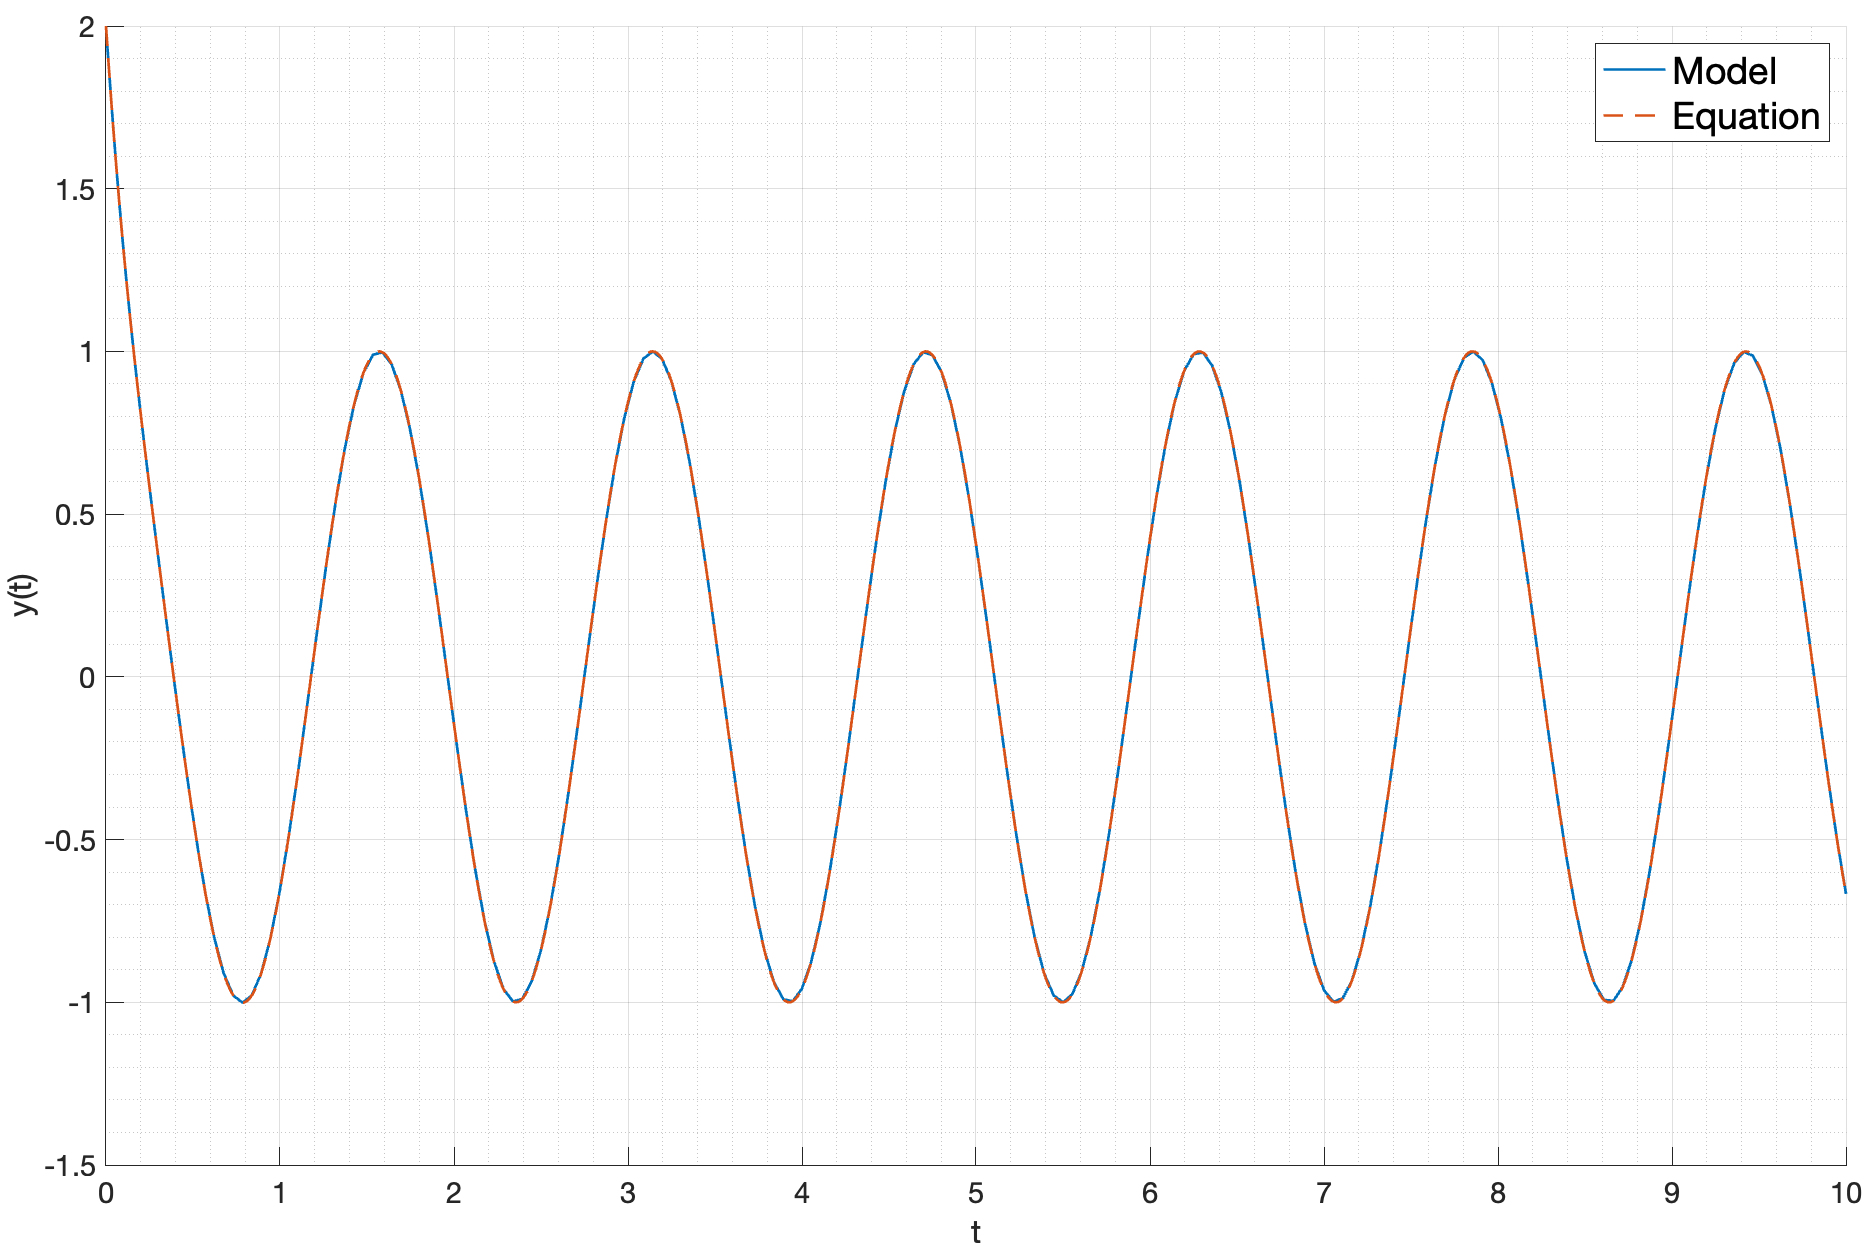
\includegraphics[width=\textwidth]{media/generator.png}
    \caption{Результат моделирования автономного генератора}
    \label{fig:autonomous_generator_simulation}
\end{figure}

\subsection{Вывод}
В ходе выполнения данной работы была рассмотрена система с комплексными собственными числами. 
Мне удалось найти такие параметры системы, при которых выход системы принимает желаемый вид. 
Симуляция системы в Matlab показала, что результаты моделирования совпадают с ожидаемыми. 
Для нахождения матрицы $A$ были использованы собственные числа, полученные из корней характеристического уравнения. 
Векторы $C$ и $x(0)$ были выбраны таким образом, чтобы выход системы принял желаемый вид.  
Можно сделать вывод о том, что корни характеристического уравнения соответствуют корням 
матрицы $A$. 